% !TEX root = ../master_thesis.tex
\chapter{Compléments au chapitre~\ref{chap:défauts}}\label{annexe:M}

\section{Vérifications de la matrice de couplage électron-défaut}\label{sec:annexe_M_tests}

Cette section rassemble les vérifications de la chaîne de calcul de la matrice $M$ du chapitre~\ref{chap:défauts} qui justifient un paramètre numérique : la convergence de l'interpolation en $R_\text{cut}$ et les tests de cohérence interne.
\vspace*{\fill}
\begin{table}[htbp]
    \centering
    \small
    \setlength{\tabcolsep}{3pt}
    \caption[Erreur de troncature sur les éléments de
    matrice interpolés.]{Écart relatif maximal entre les éléments de
    matrice interpolés sur une grille de sortie $60\times60$ avec troncature de
    la somme~\eqref{eqn:M_interp} à $R',R \le R_\text{cut}$, où $R$ et $R'$ sont des normes euclidiennes d'indices réduits, et ceux
    obtenus avec toutes les cellules unitaires de la représentation réelle, pour les
    super-cellules $9\times9$ et $12\times12$, sur les valeurs singulières
    des blocs $\pi$--$\pi^*$ et sur les éléments
    diagonaux $M_{nn}(\kv,\kv)$, avec les matrices brutes et alignées (section~\ref{sec:M_détails}). La deuxième colonne donne le nombre de
    cellules unitaires retenues.}
    \label{tab:rcut_M}
    % Généré par scripts/make_tables.py : ne pas éditer (python scripts/make_tables.py --only rcut_M).
% tab:rcut_M, §4.1.5 → annexe D. Valeurs et sources cellule par cellule : tables/SOURCES.md.
% Sources : M2_plateau/m_rcut_convergence.csv ; kaasbjerg/r10_c2_results.json
\begin{tabular}{c c cc cc cc cc}
    \hline\hline
    & & \multicolumn{4}{c}{$9\times9$} & \multicolumn{4}{c}{$12\times12$} \\
    \cline{3-6}\cline{7-10}
    & & \multicolumn{2}{c}{brut} & \multicolumn{2}{c}{aligné} & \multicolumn{2}{c}{brut} & \multicolumn{2}{c}{aligné} \\
    $R_\text{cut}$ & Cellules & $\pi$--$\pi^*$ & diag. & $\pi$--$\pi^*$ & diag. & $\pi$--$\pi^*$ & diag. & $\pi$--$\pi^*$ & diag. \\
    \hline
    0 & 1   & 32~\%   & 26~\%   & 32~\%   & 32~\%  & 99~\%  & 85~\%  & 99~\%  & 87~\% \\
    1 & 5   & 19~\%   & 23~\%   & 19~\%   & 15~\%  & 20~\%  & 24~\%  & 19~\%  & 19~\% \\
    2 & 13  & 13~\%   & 12~\%   & 6.6~\%  & 4.6~\% & 15~\%  & 14~\%  & 13~\%  & 13~\% \\
    3 & 29  & 8.8~\%  & 7.2~\%  & 2.6~\%  & 1.7~\% & 12~\%  & 10~\%  & 3.3~\% & 3.1~\% \\
    4 & 49  & 5.8~\%  & 4.8~\%  & 2.0~\%  & 1.4~\% & 10~\%  & 8.4~\% & 2.5~\% & 1.5~\% \\
    5 & 81  & 1.4~\%  & 1.6~\%  & 1.1~\%  & 1.2~\% & 6.9~\% & 5.9~\% & 1.6~\% & 0.85~\% \\
    6 & 113 & 0.85~\% & 0.97~\% & 0.92~\% & 1.0~\% & 3.8~\% & 3.6~\% & 1.1~\% & 0.87~\% \\
    \hline\hline
\end{tabular}

\end{table}
\vspace*{\fill}
\clearpage
\vspace*{\fill}
\begin{figure}[htbp]
    \centering
    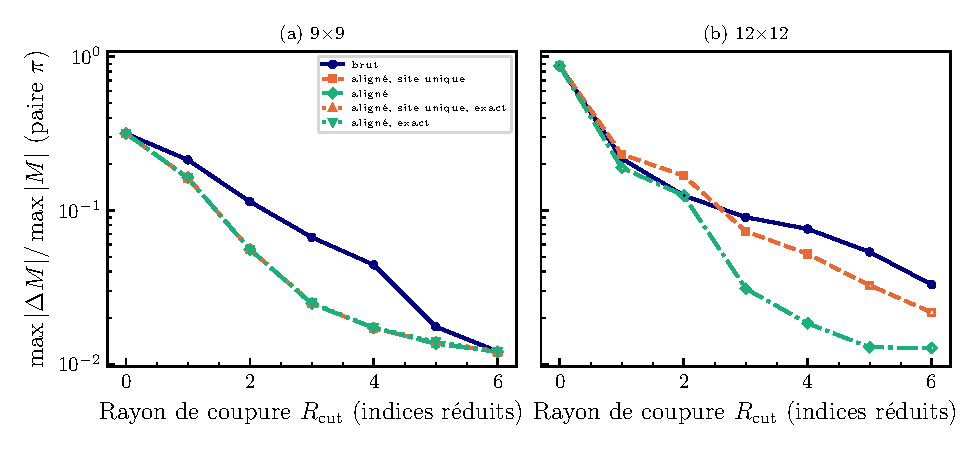
\includegraphics[width=\textwidth]{figures/fig_rcut_aligned.pdf}
    % À REVOIR : légende provisoire du 2026-10-05 ; étiquettes « site unique » / « Kumagai–Oba » de la figure à renommer (make_figures_controles.py)
    \caption[Erreur de troncature selon la référence du potentiel.]{Écart relatif maximal $\max|\Delta M|/\max|M|$ sur les blocs $\pi$--$\pi^*$ entre les éléments de matrice interpolés avec troncature à $R_\text{cut}$ et ceux obtenus avec toutes les cellules, pour (a) $9\times9$ et (b) $12\times12$, avec les matrices brutes, les matrices alignées de production (constante de Kumagai-Oba) et une variante alignée sur un seul site ; les courbes « exact » appliquent l'alignement au potentiel plutôt qu'aux blocs diagonaux de la base de Wannier et se superposent aux précédentes. C'est la quantité de la première ligne du tableau~\ref{tab:rcut_M}, pour tous les rayons de coupure.}
    \label{fig:rcut_aligned}
\end{figure}
\vspace*{\fill}
\clearpage
\begin{figure}[htbp]
    \centering
    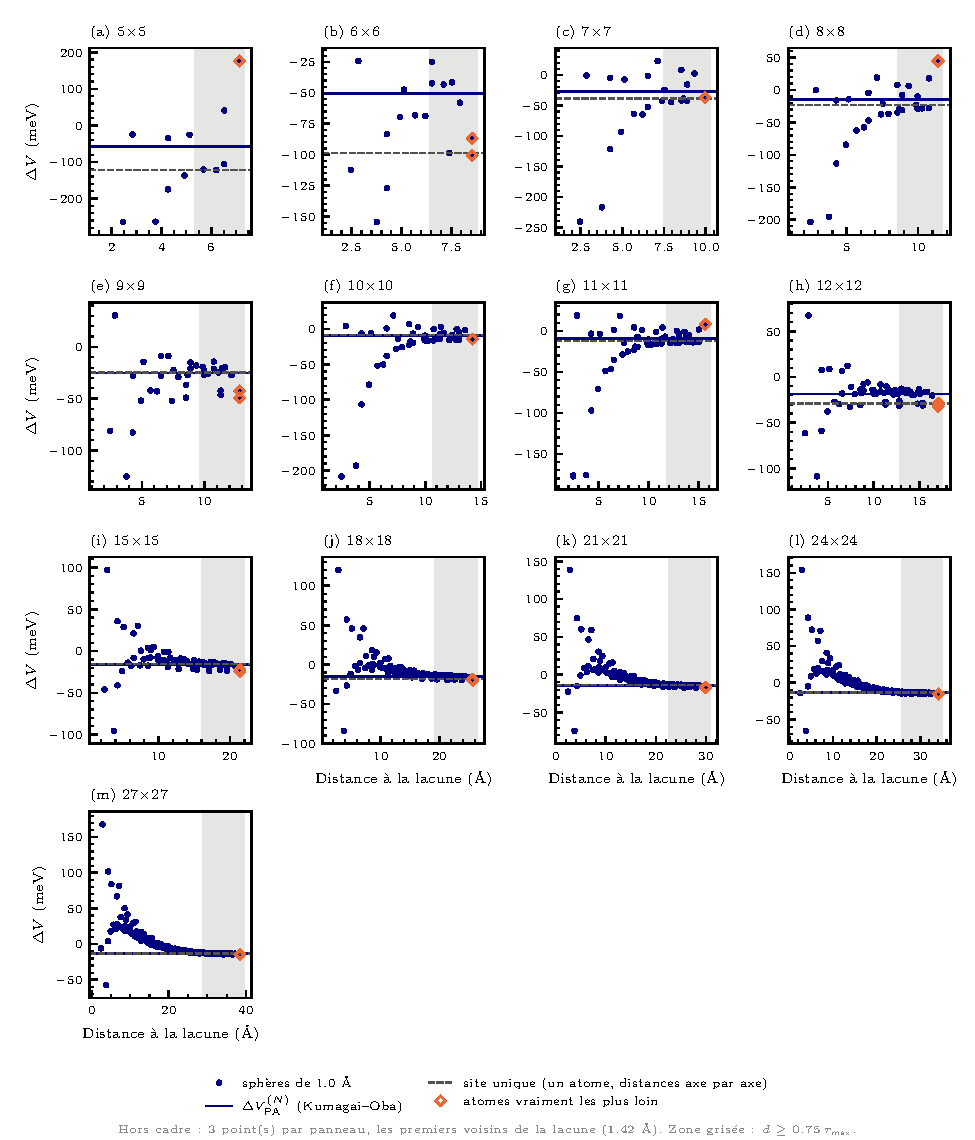
\includegraphics[width=\textwidth]{figures/fig_offset_profiles_13.pdf}
    % À REVOIR : légende provisoire du 2026-10-05 ; étiquettes « Kumagai–Oba » / « site unique » de la figure (make_figures_controles.py)
    \caption[Décalages de potentiel sur les sites atomiques pour treize tailles.]{Décalage du potentiel de la lacune $\Delta V_\alpha$ moyenné sur une sphère de $1.0$~\AA{} autour de chaque atome, en fonction de la distance à la lacune (image minimale), pour les treize tailles de super-cellule de $5\times5$ à $27\times27$. La zone grisée marque la région $d\ge0.75\,r_\text{max}$ dont la moyenne définit la constante d'alignement $\Delta V_\text{PA}^{(N)}$ (trait plein, prescription (A) du tableau~\ref{tab:alignement}) ; les tirets donnent la valeur du site unique le plus éloigné (prescription (D)) et les losanges marquent les atomes les plus éloignés.}
    \label{fig:offset_profiles_13}
\end{figure}
\clearpage
\vspace*{\fill}
\begin{figure}[htbp]
    \centering
    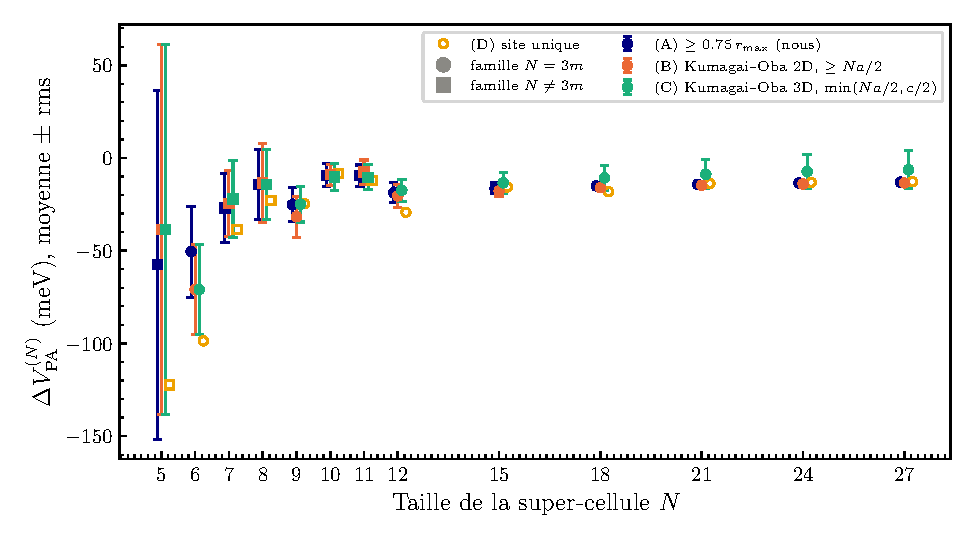
\includegraphics[width=\textwidth]{figures/fig_alignement_regions.pdf}
    % À REVOIR : légende provisoire du 2026-10-05
    \caption[Constante d'alignement selon la région d'échantillonnage.]{Constante d'alignement $\Delta V_\text{PA}^{(N)}$ (moyenne et écart-type des décalages de sphère) en fonction de la taille $N$ de la super-cellule, pour les quatre prescriptions du tableau~\ref{tab:alignement} : (A) $d\ge0.75\,r_\text{max}$ (production), (B) Kumagai-Oba à deux dimensions, $d\ge Na/2$, (C) Kumagai-Oba à trois dimensions, $d\ge\min(Na/2, c/2)$, et (D) site unique.}
    \label{fig:alignement_regions}
\end{figure}
\vspace*{\fill}
\clearpage
\vspace*{\fill}
\begin{figure}[htbp]
    \centering
    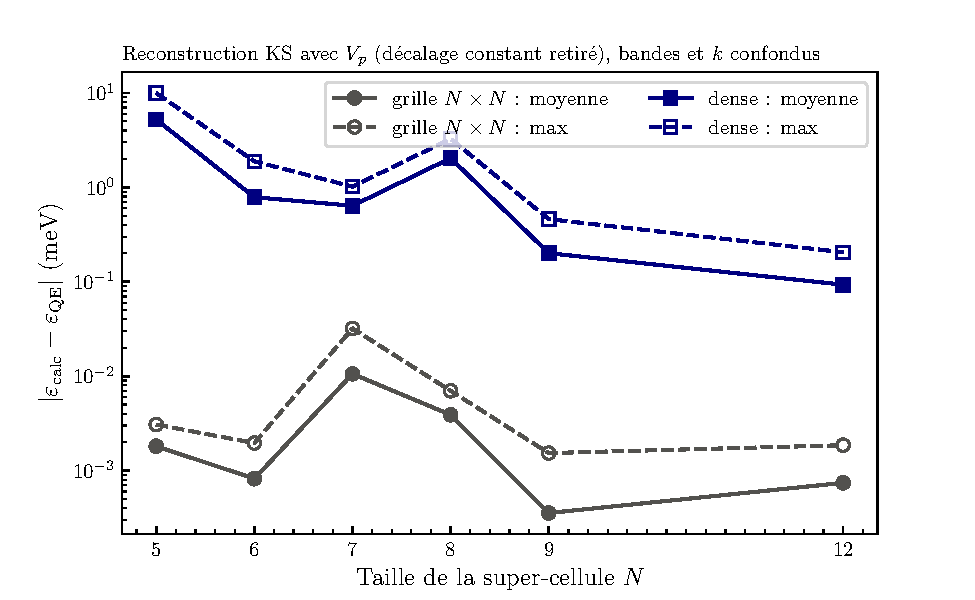
\includegraphics[width=\textwidth]{figures/fig_ks_reconstruction.pdf}
    \caption[Reconstruction des valeurs propres de Kohn-Sham.]{Écart
    entre les valeurs propres de Kohn-Sham reconstruites par la chaîne
    d'évaluation des éléments de matrice, appliquée au potentiel de la
    super-cellule parfaite, et celles de \texttt{QuantumESPRESSO}.
    La moyenne et le maximum sont sur toutes les bandes et tous les points $\kv$, après le retrait d'un décalage constant entre les deux références d'énergie. L'exercice est fait pour les grilles $N\times N$, où la densité convergée est la même pour les états et le potentiel, et pour les grilles élargies $pN\times pN$, où la densité autocohérente est différente.}
    \label{fig:ks_reconstruction}
\end{figure}
\vspace*{\fill}
\clearpage
\vspace*{\fill}
\begin{table}[htbp]
    \centering
    \small
    \setlength{\tabcolsep}{2pt}
    % À REVOIR : légende provisoire du 2026-10-03
    \caption[Vérifications de la chaîne de calcul de la matrice de
    couplage.]{Vérifications de la chaîne de calcul de la matrice $M$ : les tests et la quantité qu'ils contrôlent, la valeur obtenue et le seuil d'acceptation. Sauf mention contraire la valeur est celle de la super-cellule de référence $9\times9$ ; les reconstructions de Kohn-Sham, l'hermiticité et l'application directe de $V_\text{ed}$ sont données en fourchette ou en maximum sur les six tailles, et le test de convention intensive porte sur chaque famille de tailles.}
    \label{tab:tests_M}
    \begin{tabular}{l l l l}
    \hline\hline
    Test & Quantité & Valeur & Seuil \\
    \hline
    Reconstruction KS, grille $N\times N$             & $\max|\varepsilon_\text{calc}-\varepsilon_\text{QE}|$ & 1.5--32~$\mu$eV            & --- \\
    \quad éléments hors diagonaux                     & rel. à $\max|\varepsilon|$                            & $\le 1.3\times10^{-6}$     & --- \\
    Reconstruction KS, grille élargie                 & $\max|\varepsilon_\text{calc}-\varepsilon_\text{QE}|$ & 0.21--10~meV               & --- \\
    Hermiticité ($M$ élargi, six tailles)             & $\max|M-M^\dagger|/\max|M|$                           & $\le 2.3\times10^{-14}$    & $10^{-12}$ \\
    Application directe de $V_\text{ed}$, $N\times N$ & $\max|\Delta M|$, L et NL                             & $\le 3.3\times10^{-14}$~eV & $10^{-6}$~eV \\
    \quad grilles élargies                            & idem                                                  & $\le 1.2\times10^{-8}$~eV  & $10^{-6}$~eV \\
    Remplissage, coefficients coïncidents             & $\max|\Delta M^\text{L}|/\max|M^\text{L}|$            & $1.3\times10^{-15}$        & $10^{-10}$ \\
    Remplissage, points $\kv$ communs                 & écart rel. valeurs singulières                        & $1.3\times10^{-3}$         & $2\times10^{-3}$ \\
    Fourier $\kv\to\Rv\to\kv$                         & $\max|\Delta M|/\max|M|$                              & $2.4\times10^{-14}$        & $10^{-12}$ \\
    Bloch$\to$Wannier$\to$Bloch                       & écart rel. valeurs singulières                        & $1.3\times10^{-15}$        & $10^{-12}$ \\
    Convention intensive, $N = 6, 9, 12$              & $(\max-\min)/\text{moy.}$ de $\max|M|$                & $2.3\times10^{-2}$         & $5\times10^{-2}$ \\
    \quad $N = 5, 7, 8$                               & idem                                                  & $2.1\times10^{-2}$         & $5\times10^{-2}$ \\
    \hline\hline
\end{tabular}

\end{table}
\vspace*{\fill}
\clearpage
\section{Paramètres de calcul}\label{sec:annexe_param_M}
\vspace*{\fill}
\begin{table}[htbp]
    \centering
    \caption[Paramètres des fonctions de Wannier.]{Paramètres des fonctions de Wannier de la cellule unitaire, pour la chaîne de la matrice $M$ (chapitre~\ref{chap:défauts}) et la chaîne de la matrice $g$ (chapitre~\ref{chap:eph}).}
    \label{tab:param_wannier}
    \small
    \setlength{\tabcolsep}{4pt}
    \begin{tabular}{p{0.27\textwidth} p{0.46\textwidth} p{0.14\textwidth}}
        \hline\hline
        Paramètre & Valeur & Section \\
        \hline
        Code (chaîne $M$) & \texttt{Wannier90} & \ref{sec:M_détails} \\
        Code (chaîne $g$) & \texttt{EPW}, qui fait appel à \texttt{Wannier90} & \ref{sec:g_détails} \\
        Grille (chaîne $M$) & grille élargie $pN\times pN$, soit $27\times 27$ pour la super-cellule de référence $9\times 9$ & \ref{sec:M_détails} \\
        Grille (chaîne $g$) & $24\times 24$ & \ref{sec:g_détails} \\
        Nombre de fonctions de Wannier & $5$ & \ref{sec:M_détails}, \ref{sec:g_détails} \\
        Fonctions d'essai & trois orbitales hybrides $sp^2$ et une orbitale $p_z$ sur un atome de carbone, une orbitale $p_z$ sur l'autre & \ref{sec:M_détails}, \ref{sec:g_détails} \\
        Fenêtre externe & $-25$~eV à $15$~eV & \ref{sec:M_détails}, \ref{sec:g_détails} \\
        Fenêtre gelée & jusqu'à $E_D + 2.5$~eV & \ref{sec:M_détails}, \ref{sec:g_détails} \\
        Étalements (chaîne $M$) & $0.61095$~\AA$^2$ ($\sigma$), $0.96695$~\AA$^2$ ($p_z$), total $3.76675$~\AA$^2$ & \ref{sec:M_détails} \\
        Étalements (chaîne $g$) & $0.6106$~\AA$^2$ ($\sigma$), $0.9655$~\AA$^2$ ($p_z$), total $3.7627$~\AA$^2$ & \ref{sec:g_détails} \\
        \hline\hline
    \end{tabular}
\end{table}
\vspace*{\fill}
\vspace*{\fill}
\begin{table}[htbp]
    \centering
    \caption[Paramètres des super-cellules et de la matrice $M$.]{Paramètres des calculs de super-cellules et de la matrice de couplage électron-défaut $M$ (chapitre~\ref{chap:défauts}).}
    \label{tab:param_M}
    \small
    \setlength{\tabcolsep}{4pt}
    \begin{tabular}{p{0.27\textwidth} p{0.46\textwidth} p{0.14\textwidth}}
        \hline\hline
        Paramètre & Valeur & Section \\
        \hline
        Tailles de super-cellule $N\times N$ & $N = 5, 6, 7, 8, 9, 12$ ; référence $9\times 9$ & \ref{sec:M_détails}, \ref{sec:M_results} \\
        Sous-réseau de la lacune & A pour $N = 5, 7, 8, 9$ ; B pour $N = 6, 12$ & \ref{sec:M_détails} \\
        Géométrie & non relaxée & \ref{sec:M_détails} \\
        Échantillonnage de la super-cellule & point $\Gamma$ seul & \ref{sec:M_détails} \\
        Grille grossière & $N\times N$ & \ref{sec:M_détails} \\
        Facteur d'élargissement $p$ & $5, 4, 4, 4, 3, 2$ pour $N = 5, 6, 7, 8, 9, 12$ & \ref{sec:M_détails} \\
        Grille élargie $pN\times pN$ & $pN = 25, 24, 28, 32, 27, 24$ & \ref{sec:M_détails} \\
        Fonctionnelle d'échange-corrélation & PBE & \ref{sec:M_détails} \\
        Pseudo-potentiel & ONCV \textit{stringent} pour le carbone, forme de Kleinman-Bylander, bibliothèque PseudoDojo & \ref{sec:M_détails} \\
        Coupure $E_\text{cut}$ & $100$~Ry & \ref{sec:M_détails} \\
        Occupation & Marzari-Vanderbilt, $\sigma = 0.01$~Ry & \ref{sec:M_détails} \\
        Seuil de convergence & $10^{-10}$~Ry sur l'énergie totale (super-cellules), $10^{-14}$~Ry (cellule unitaire) & \ref{sec:M_détails} \\
        Cellule de vide & $30$~Bohr & \ref{sec:M_détails} \\
        Troncature de Coulomb & bidimensionnelle & \ref{sec:M_détails} \\
        Rayon de coupure $R_\text{cut}$ & $3$, soit $29$ cellules unitaires & \ref{sec:M_results} \\
        Grille de sortie du test de troncature & $60\times 60$ & \ref{sec:M_results} \\
        Nombre de bandes & super-cellules : $2N^2$ bandes occupées et $30$ bandes vides ($N\le 18$) ou $5~\%$ de plus ($N\ge 21$), deux de moins avec la lacune ; cellule unitaire : $16$ (SCF) et $20$ (NSCF des grilles $\ge 24\times 24$) & \ref{sec:M_détails} \\
        Alignement du potentiel & Kumagai-Oba : moyenne des décalages de sphères de $1.0$~\AA{} sur les atomes à distance $d \ge 0.75\,r_\text{max}$ de la lacune (image minimale) ; soustrait des blocs diagonaux $M(\Rv,\Rv)$ des $N^2$ cellules dans la base de Wannier & \ref{sec:M_détails} \\
        Constante d'alignement $\Delta V_\text{PA}^{(N)}$ & $-57.6$, $-50.5$, $-26.9$, $-14.4$, $-25.1$, $-18.7$~meV pour $N = 5, 6, 7, 8, 9, 12$ ; incertitude $9.05$~meV pour $9\times 9$ & \ref{sec:M_results} \\
        \hline\hline
    \end{tabular}
\end{table}
\vspace*{\fill}
